\subsection{Rate Encoding}

Lets try and see how to to encode Mnist digit data set via Rate Encoding specified in \ref{ssec:rate-encoding}.

By using equation \ref{eq:rate-enc-prob}, we can implement the rate encoding approach in a way that controls the spike generation based on the input image and ensures that high-intensity pixels (corresponding to higher values of \(f(x_{i,j})\)) will appear in more patterns.

Overall, the rate encoding approach, combined with the derived probability constraints and stochastic spike generation, enables us to effectively convert an image into a time-varying sequence of spikes while preserving its features. This method allows us to model the behavior of real neurons and capture the temporal dynamics of the input information, making it suitable for various applications in neural information processing and spiking neural network simulations.

\begin{figure}[H]
    \centering
    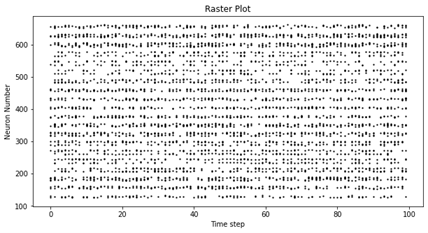
\includegraphics[width=0.5\textwidth]{methods/spike-encoding/graphs/rate-encoding-raster.png}
    \caption{Raster plot of a random Mnist image encoded via Rate Encoding with maximum rate of 20 Hz over trial time of 1 sec}
    \label{fig:rate-encoding-raster}
\end{figure}
